\cleardoublepage

\section{绪论}

\subsection{研究背景与意义}

随着计算机科技的不断发展,各种计算机技术已经成为人们生活不可或缺的一部分,聊天软件、移动支付、影音技术都为日常生活带来极大的便捷。但是,这些技术在带来便捷的同时也导致了越来越多的安全问题。2021年4月,超过5.3亿Facebook用户的数据被泄露,其中包括姓名、出生日期、社交关系等敏感信息。2022年6月,西北工业大学发布声明称遭受境外的网络攻击,导致被窃取部分敏感信息。2023年6月,苹果iOS操作系统被曝存在安全漏洞,可能导致用户手机被黑客完全控制。由此可见,网络安全已经成为不可忽视的问题,个人的隐私及安全由此受到严重的威胁。因此需要尽量减少计算机系统中的漏洞,在让人们享受便捷的同时能够保护个人隐私安全。

与此同时,由于摩尔定律逐渐接近极限,多核处理器由于其对性能的提升被广泛地使用。相应地,由于并发编程模式能够充分发挥多核处理器的性能,因此也被编程人员青睐,合理的并发编程可以的大大提升程序运行的效率。但是这也引入了和顺序程序不同的安全漏洞,当并发程序不正确地处理多个线程之间的同步时就会导致并发错误,进而导致并发漏洞,黑客可以通过这些漏洞对系统发起攻击。例如,当多个线程对同一个变量的访问没有受到保护时,由于运行过程中线程执行的序列不同,最后变量的值被错误地更改,导致漏洞的产生。

目前已经有多种并发漏洞检测手段,包括静态检测、符号执行、模糊测试等,但是静态分析存在着准确率低,误报率高的缺点;符号执行的开销则会随着程序复杂度的提升迅速增大,而模糊测试可以在保证准确率的同时以可接受的开销来挖掘漏洞。随着计算机性能的提升以及AFL-ref的提出,模糊测试成为挖掘漏洞的重要手段。模糊测试最早由Barton Miller提出,最初用来测试程序的健壮性,后来才逐渐用于进行漏洞挖掘,模糊测试技术经过多次重要的发展,现在已经逐渐完善并得到广泛应用。但是由于并发程序的复杂性以及运行时的不确定性,并发漏洞能够被触发的概率很小,导致检测并发漏洞并稳定复现仍然存在困难。

当前通用的模糊测试工具只能处理通用地程序输入,而不能扩展到程序并发执行的维度,尽管目前存在一些对并发程序进行模糊测试的工作,但是都存在一定的局限性。因此本文主要探究将模糊测试应用在并发漏洞挖掘上,以实现高效的并发漏洞挖掘。


\subsection{国内外研究现状}

\subsubsection{利用部分顺序规约进行并发漏洞挖掘}

并发程序中线程或者进程的执行可能以多种方式交织,如果直接进行探索会导致状态空间呈指数级增长,在有状态的情况下甚至会造成状态爆炸,这对于当前的计算能力来说是不现实的,计算机无法在合理时间内对如此大量的情况进行探索,因此有必要提出一种能够减少并发程序探索空间的技术。部分顺序规约作为一种检查各个状态和行为间的独立性以减小整体的状态空间的技术,正好可以应用到并发漏洞挖掘,通过识别关键数据的依赖关系,将等价的并发程序交织归约到同一个集合,每一个集合只需要执行一次就可以对集合中的所有情况进行检测。

早在2005年,Flanagan\cite{flanagan2005dynamic}等人通过动态地跟踪进程间的相互作用,识别出需要回溯的点,从而探索状态空间中的替代路径。最终结果显示动态的部分顺序规约可以在线程不断增多的情况下避免状态爆炸的产生。

2014年,Abdulla\cite{abdulla2014optimal}等人提出了一种新的动态部分顺序规约算法并实现工具optimal-DPOR,通过引入源集合记录当前某个调度点上的所有可能的操作,避免探索与已探索的执行等价的执行路径,从而减少冗余探索。同时这篇文章还引入了唤醒树机制,控制未来探索的初始步骤,确保算法不会遇到任何睡眠集阻塞的探索。最终实验结果显示,optimal-DPOR在导致不超过10\%开销的情况下加速了并发空间的探索。

2019年,Abdulla\cite{abdulla2019optimal}等人提出了首个针对顺序一致性语义下的多线程程序的无状态模型检查算法,算法基于一种更粗粒度的等价关系——reads-from,这种关系保留了从写操作到读操作的依赖关系,但放宽了对执行顺序的要求。通过精确地探索每个“reads-from”等价类中的一个执行路径,避免对等价的执行路径进行重复探索。根据这个算法,作者实现了Nidhugg/rfsc并进行了大量测试,首先,Nidhugg/rfsc在某些情况下比最快的SMC工具慢,但在其他情况下,它在探索执行数量上的性能要么类似,要么更好,并且在某些程序中比其他工具快指数级。其次,在测试的49个程序中,Nidhugg/rfsc在大多数程序中找到了bug,并且在其中一些程序中,它是唯一能够找到bug的工具。通过进一步分析,Nidhugg/rfsc可以正确地识别出多线程程序中的reads-from relation。

\subsubsection{利用模糊测试进行漏洞挖掘}

2019年,Jeong\cite{jeong2019razzer}等人开发了Razzer,通过静态分析(point-to analysis)识别,得到所有可能产生冲突的指令对,就是可能访问同一个地址的属于不同线程的两条指令,并得到所有可能产生冲突的指令对集合。然后进行单线程模糊测试以得到可以使程序执行到特定访存指令的输入。然后进行多线程测试,利用单线程测试得到的输入以及断点插入,使得程序按照规划好的顺序交错执行,然后观察是否会让程序发生异常或者其他错误。相比于Syzkaller,这一方法可以用更少的变异、执行次数找到更多的有效bug。但是Razzer的执行速度相比于Syzkaller更慢,并且利用point-to-analysis可能无法找到所有的冲突指令对。

2020年,Hongxu Chen\cite{chen2020muzz}等人提出了MUZZ,这篇文章首先通过静态分析得到可能会产生冲突的scope,然后对这些scope进行插桩。然后进行fuzzing的过程,利用前面插桩 的代码,得到代码覆盖率,线程上下文,交错顺序三个信息,并根据这些信息进行种子的选择,排序,变异,生成新的测试用例。最后利用T-Sanitize检测漏洞。相比于之前的 工作,MUZZ能够产生出更多和多进程相关的种子,也就是说能够测试更多多线程的用例。 同时相比于AFL等工具能够检测出更多的数据争用缺陷.。

2020年,Meng Xu\cite{xu2020krace}等人提出了KRACE,通过引入一个新的覆盖跟踪指标,别名覆盖率,来捕获并发维度的探索进度。通过这个新的维度,结合一种用于生成、变异、合并多线程 系统调用序列的进化算法,引导fuzzer对线程并发空间进行更有效的探索。相对于Syzkaller,KRACE可以发现更多的branch path。但是也会引入更大的开销。 

2022年,Zu-Ming Jiang\cite{jiang2022context}等人通过引入并发调用对这个新的并发覆盖指标,确保上 下文敏感性,并提出了一种邻接导向突变,生成新的可能的线程交错。这篇文章提出了 CONZZER 框架,并在8个用户级程序和4个内核级文件系统上进行了测试,并发现了95个数据竞争,其中75个是有害的。 

2023年,Jeong等人提出SEGFUZZ\cite{jeong2023segfuzz},将对整个线程的交错空间进行分解,对一小段代码进行探索,然后再将多个小段代码合并再进行探索,并提出交织段覆盖率的概念,再提高发现并发错误的准确性的同时,避免了冗余测试。这很大程度上降低了并发空间探索的复杂度。SEGFUZZ在linux内核中发现了21个新的并发错误,并且这些错误都表现出有害行为。并且相对于 Snowboard和KRACE这些之前的工作能够更快地发现并发错误(平 均快 4.1 倍)。 

2023年,Ming Yuan等人开发了DDRACE\cite{yuan2023ddrace},提出了新的距离度量反馈,RPIP(Race Pair Interaction Profile)反馈,约束反馈,来指导生成新的输入,并利用一种交错优先级 方案来选择更有可能产生并发访问缺陷的输入。相对于Syzkaller,RAZZER,KRACE这些工具,DDRACE可以发现更多的并发访问缺陷,并且可以在更短时间内发现。


\subsection{论文主要研究内容}

对本论文的主要工作进行叙述,包括创新点,所作的实验,所有的可以用来作为工作量的东西都放上去

\subsection{论文的组织方式}

对每一章写了些什么进行叙述,这个可以等到后面写完了再来补充,避免会进行调整



\section{背景知识}



本章对相关的背景知识进行详细的介绍。第一个部分是对并发漏洞的介绍,对常见的并发漏洞模式进行梳理,指出其特点。然后整体介绍通用模糊测试,然后介绍模糊测试究竟是什么,其利用到的一些技术。

\subsection{竞争条件}

\subsubsection{竞争条件的产生}

竞争条件是指电子设备、软件或者其他系统的实质性行为取决于其他不可控的顺序或者时间,从而导致意外或者不一致的结果。如果其中一种或者多种行为是不能接受的 情况,它就会成为一个漏洞。其中关键的就是其输出的不确定性,正常情况下计算机会按照编写的代码严格地执行,就像数学中的逻辑一样严谨,给定同一个输入,那么任意次的测试中,系统都会有相同的输出。但是对于多线程程序,同样的输入,却有可能导致不同的输出结果。为了简单起见,这里讨论单核情况下的多线程程序。

\begin{lstlisting}[%
    language={C},
    caption={simple.c},
    label={code:racecondition},
]
int a = 0;
int thread1(){
    // ...
    reg = a; 			(1)
    reg = reg + 1;		(2)
    a = reg;			(3)
    // ...
}
int thread2(){
	// ...
	reg = a;			(4)
	reg = reg - 1;		(5)
	a = reg;			(6)
	// ...
}
\end{lstlisting}

假设一个程序\autoref{code:racecondition}包含两个线程,两个线程都会访问同一个变量a,线程1将a增加1,线程2将a减去1。那么就会出现以下几种情况:

\begin{enumerate}
\item $(1) \Rightarrow (2) \Rightarrow (3) \Rightarrow (4) \Rightarrow (5) \Rightarrow (6)$
\item $(1) \Rightarrow (2) \Rightarrow (4) \Rightarrow (3) \Rightarrow (5) \Rightarrow (6)$
\item $(1) \Rightarrow (4) \Rightarrow (2) \Rightarrow (5) \Rightarrow (3) \Rightarrow (6)$
\end{enumerate}

如\autoref{fig:data_race}所示,在第一种情况下,thread1正常将a的值进行改变并写回,使a的值增加1,在写回之后thread2开始操作,将a的值减一并写回,最终a的值仍然为0,结果正确。

\begin{figure}[ht]
    \centering
    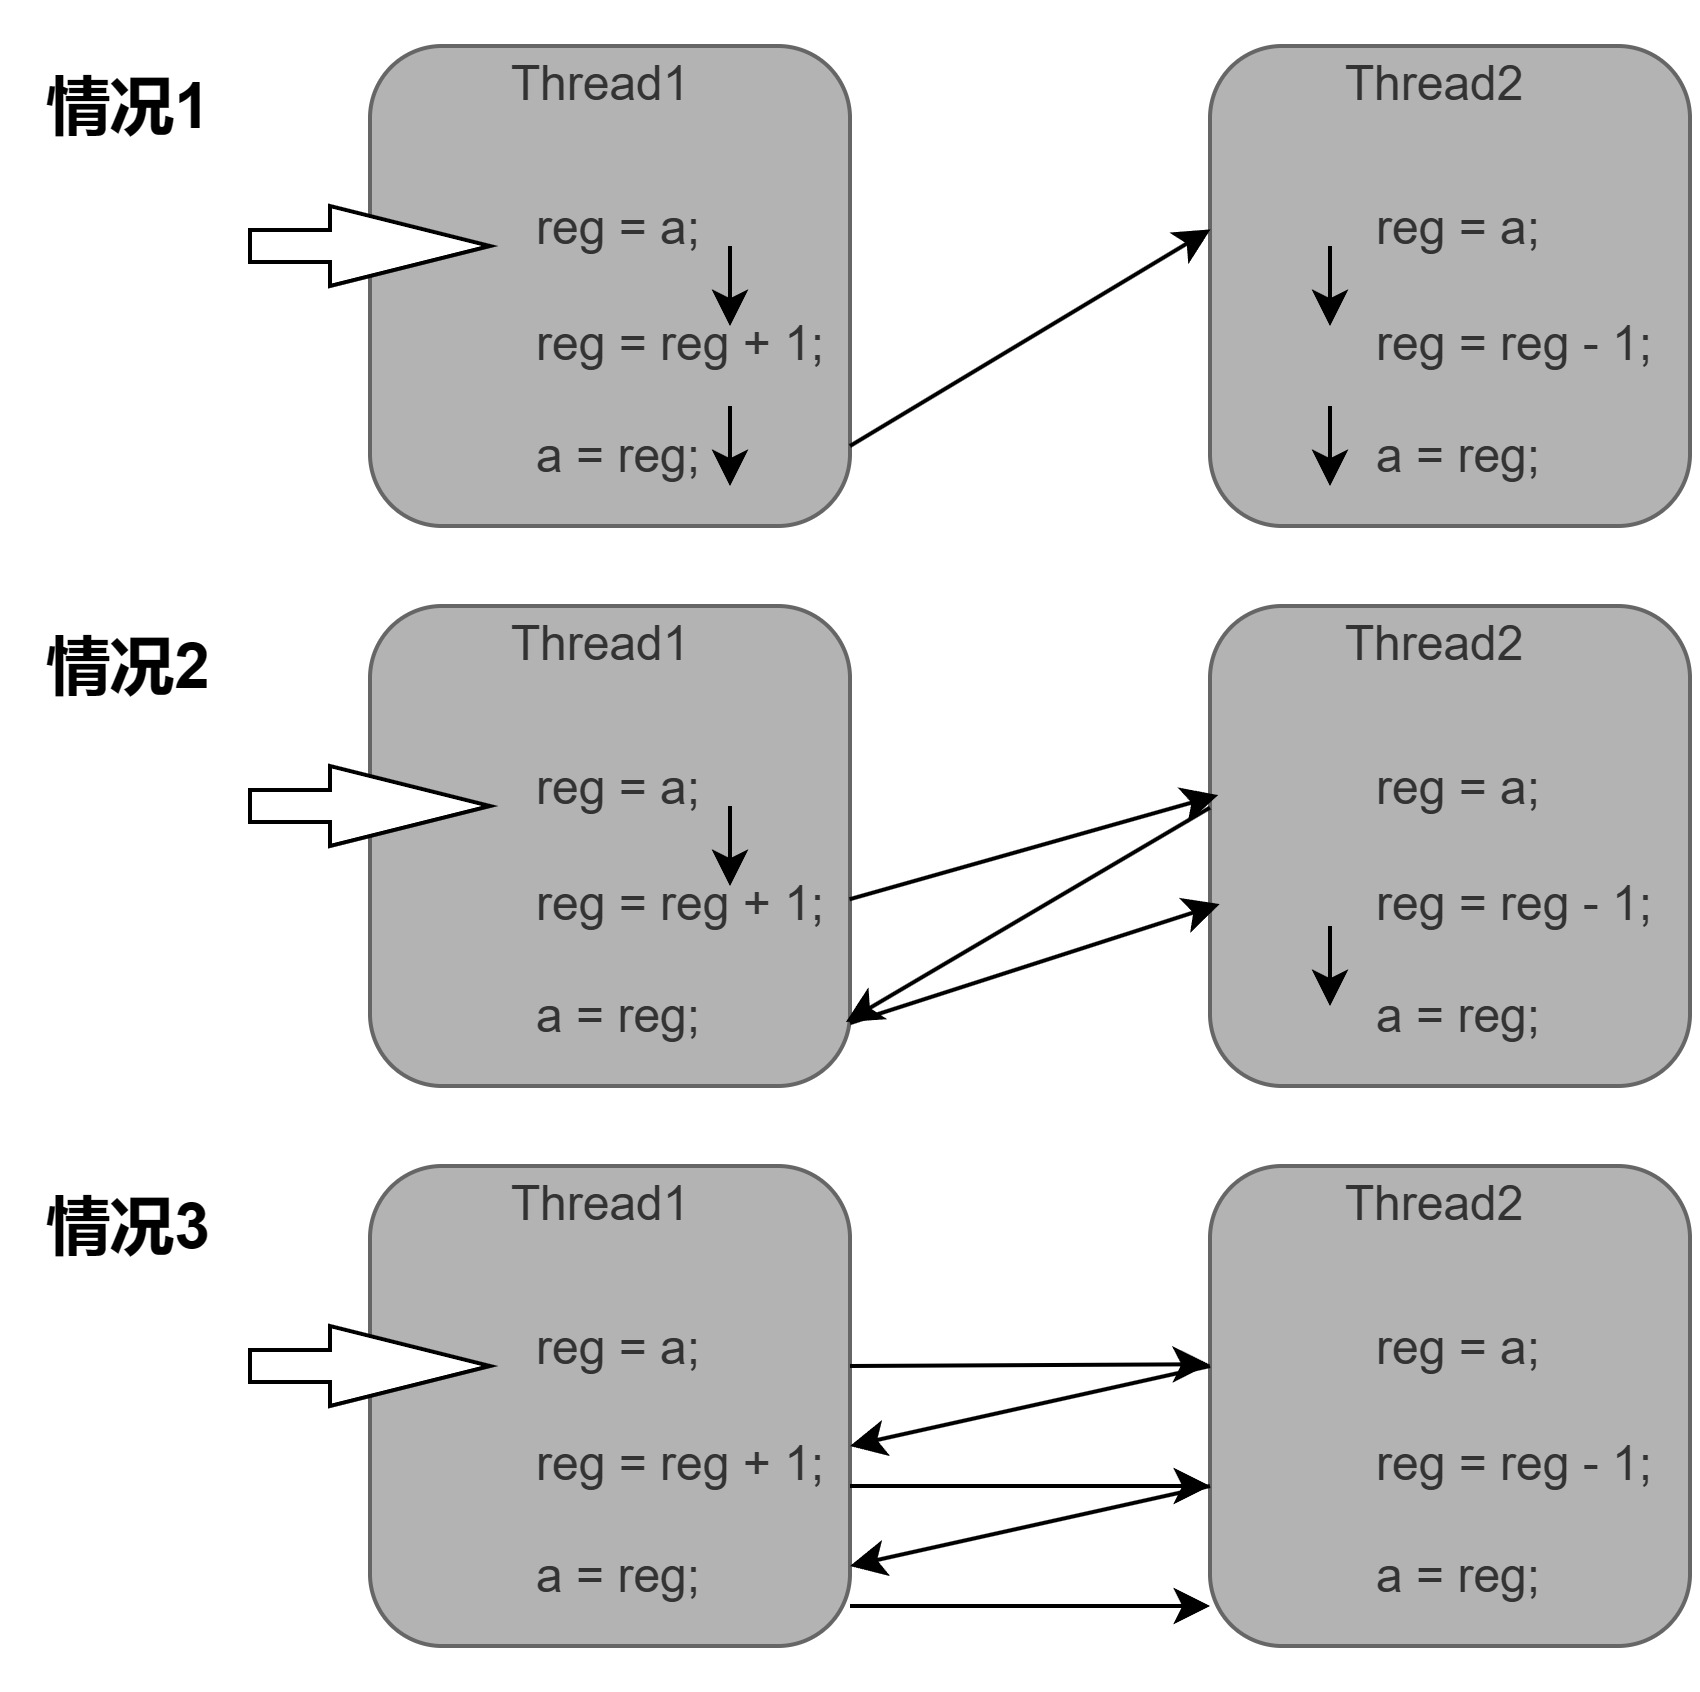
\includegraphics[width=.7\linewidth]{data_race}
    \caption{\label{fig:data_race}Data Race}
\end{figure}


在第二种情况下,thread1首先将a的值0读到reg并加1,然后thread2将a的值0读到thread2的reg中,随后thread1将1写入到a中,但是由于thread2最后直接将-1写入到a中,原本thread1写进去的1会被直接覆盖,导致得到一个错误的结果。第三种情况和第二种情况类似。

简单分析可知,发生错误的根本原因在于(4)在(3)之前发生了,这导致两个线程同时拿到了a的数据并进行处理,最终写回的时候就会出现覆盖的情况,导致错误。两个线程在他们自己线程中的处理都是正确的,但是从多个线程的视角来看,由于线程调度顺序的可能不同,每一次运行程序得到的结果都可能不一样。

而多线程程序的调度往往受随机条件影响,例如操作系统的进程调度器可能受到其他进程的影响,导致当前线程的调度出现偏差;外部的中断也可以打断线程的调度,而中断由外界的变化而引起,因此往往是随机化的,进而导致多线程调度的随机性。

\subsubsection{避免竞争条件的方式}

避免数据竞争主要要求程序员在编写多线程程序时严格遵守一些规则和原则包括但不限于同步,有序性和原子性。避免数据竞争的策略目前有很多,例如:

\begin{enumerate}
\item 首先,可以使用锁定机制确保任何时候只有一个线程访问数据。在执行读写操作之前,线程必须获得锁,读写完成后解锁。这样其他所有尝试获取锁的线程就会被阻塞,直到持有锁的线程完成操作。这种方法可以有效的防止数据竞争,但也 可能导致锁竞态和性能问题。
\item 其次,可以使用原子操作确保操作不受线程切换影响。所谓的原子操作,就是在执行中不会被线程切换打断的操作。一些编程语言提供了对原子操作的支持,如C++11中的std::atomic。
\item 然后,另一种策略是设计无共享数据的程序。既然数据竞争是由于多个线程同时访问同一块数据,那么避免共享数据就可以避免数据竞争。这种策略有时候被称为消息传递,其中线程之间通过发送消息来交换信息。每个线程有自己的数据副 本,因此不存在数据竞争。然而,这种方法可能会增加数据复制和通信的成本。
\item 最后,可以使用一些诸如事务性内存的较新的并发控制技术。在事务内存模型中,一组读取和写入被组合在一个事务中,只有当没有其他线程访问被事务使用的数据时,这个事务才能成功提交。
\end{enumerate}

以上就是防止数据竞争的一些常见策略和技术。谨记,无论使用哪种策略,在编写并 发代码时,始终需要注意数据访问的顺序和时机,以及线程如何互相影响。

\subsection{模糊测试}

模糊测试(Fuzz Testing或Fuzzing)是一种软件测试技术,它通过自动或半自动方式向系统提供无效、意外或随机的数据,并监控系统的响应,从而查找可能的错误和漏洞。模糊测试是通过大量的输入测试来检查程序是否存在异常状况,比如崩溃或者未捕获 的异常,是一种健壮性测试。模糊测试包括几个主要的步骤:

\begin{enumerate}
\item 确定目标:首先确定测试的目标,也就是要测试的软件或者系统。可以是一个网络协议,一个文件格式,或者一个具体的功能。
\item 生成模糊数据:这个步骤是通过不同的方法生成一些随机或伪随机的数据作为输入。可以是完全随机的数据,也可以基于一些规则或者模型生成。有些高级的模糊测试工具还能够理解输入的结构,并基于这个结构生成更有效的模糊数据。
\item 执行并监控:将这些模糊数据输入到被测试系统,监控系统的行为。如果系统出现异常,如崩溃或者挂起,那么就可能存在问题。
\item 分析结果:对每一个引发异常的输入数据进行分析,确定这是一个真实的漏洞,还是一个假阳性。如果是一个真实的漏洞,那么就需要进一步调查并修复。
\end{enumerate}

在模糊测试系统运行时,首先生成示例输入,然后利用输入运行程序,并在程序运行过程中进行监视,如果过程中发现异常,则将这一个输入记录下来。并利用获得的信息生成下一轮测试所需的输入,再次进行测试。在实际应用中,模糊测试通常结合了生成测试和变异测试的思想。它可以应用于各种软件系统,包括应用程序、操作系统、驱动程序、网络协议等,以帮助发现并修复潜在的安全漏洞和软件缺陷。总的来说,模糊测试是一种强大的测试方法,可以帮助提高软件系统的健壮性和安全性,尤其是对于大规模、复杂的软件系统来说,模糊测试具有重要的意义。

\subsubsection{插桩}

插桩技术指在保证原有程序逻辑完整性的基础上,在程序中插入探针,通过探针采集代码中的信息(方法本身、方法参数值、返回值等)在特定的位置插入代码段,从而收集程序运行时的动态上下文信息。这对于模糊测试来说非常有意义,因为模糊测试需要重复生成测试用例并在每一轮测试的时候选取最佳的用例运行程序,因此如何生成更好的测试用例以及最佳的测试用例的选择就可以通过收集前面运行过的程序信息来进行。具体来说,例如通过插桩收集运行时程序的代码覆盖率,通常来说,代码覆盖率越高,相应检测到bug的概率可能会更大,因此有着更高代码覆盖率的的程序会被选取并进行变异生成新的测试用例。

\subsubsection{符号执行}

\subsubsection{污点分析}